\section{Data and Calculation}
The experiment consists of two parts, which we performed.
\subsection{Estimation of Verdet's constant}
In the first part, we put the two polarisers, one in between the electromagnet and laser source and the other between the screen and the electromagnet. We rotated the second polariser axis and measured the intensity obtained. For our experiment, the number of turns per unit length was specified as $N=167.2/\text{ cm}$ and length of the glass rod is $15\text{ cm}$. The wavelength of the laser is $\lambda = 650\ \text{nm}$
\begin{table}[H]
\centering
\begin{tabular}{|c|c|c|c|c|c|}
\hline
$I$ (A) & $H=\pi NI\ \mathrm{Oe}$ & $\theta$ ($\degree$) & $\Delta \theta$ ($\degree$) & $\Delta \theta$ (min) & $V$ \\ 
\hline
0.00 & 0.00 & 296.90 & 0.00 & 0.00 & -- \\ 
0.25 & 131.25 & 296.40 & 0.50 & 30.00 & 0.02286 \\ 
0.50 & 262.50 & 295.70 & 1.20 & 72.00 & 0.02743 \\ 
0.75 & 393.76 & 295.20 & 1.70 & 102.00 & 0.02590 \\ 
1.00 & 525.01 & 294.70 & 2.20 & 132.00 & 0.02514 \\ 
1.25 & 656.26 & 294.20 & 2.70 & 162.00 & 0.02469 \\ 
1.50 & 787.51 & 293.50 & 3.40 & 204.00 & 0.02590 \\ 
1.75 & 918.76 & 292.80 & 4.10 & 246.00 & 0.02678 \\ 
2.00 & 1050.02 & 292.30 & 4.60 & 276.00 & 0.02629 \\ 
2.25 & 1181.27 & 292.00 & 4.90 & 294.00 & 0.02489 \\ 
2.50 & 1312.52 & 291.40 & 5.50 & 330.00 & 0.02514 \\ 
2.75 & 1443.77 & 290.50 & 6.40 & 384.00 & 0.02660 \\ 
3.00 & 1575.02 & 290.00 & 6.90 & 414.00 & 0.02629 \\ 
3.25 & 1706.28 & 289.40 & 7.50 & 450.00 & 0.02637 \\ 
3.50 & 1837.53 & 288.90 & 8.00 & 480.00 & 0.02612 \\ 
3.75 & 1968.78 & 288.60 & 8.30 & 498.00 & 0.02529 \\ 
\hline
\end{tabular}
\caption{Data for the experiment}
\end{table}
\noindent
From the above data, we get the mean value of the Verdet's constant to be $V_{\tund{avg.}} = 2.571\times 10^{-2}\ \text{min/Oe/cm}$. 
\begin{figure}[H]
    \centering
    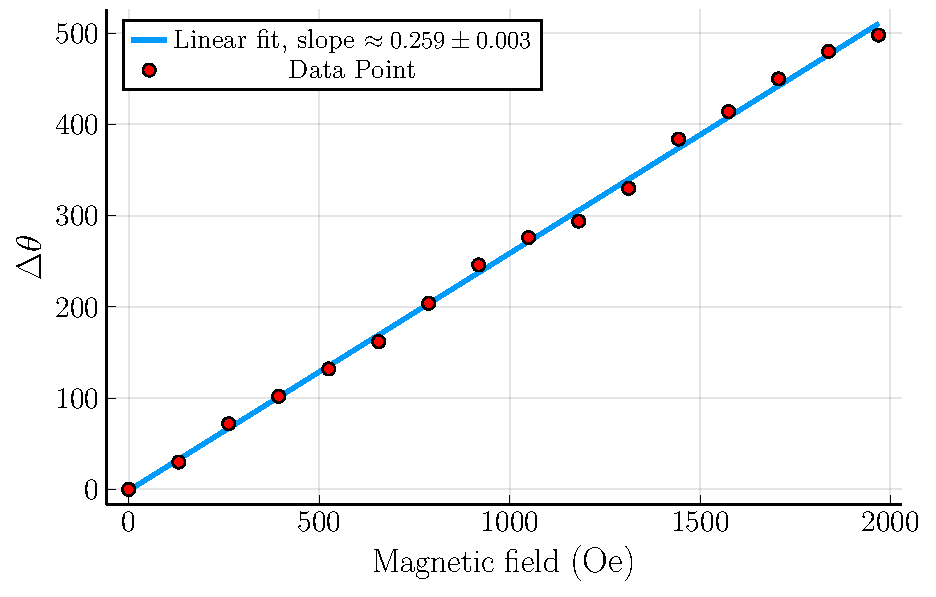
\includegraphics[width=0.7\textwidth]{verdet.pdf}
\end{figure}
\noindent
From the plot of $\Delta \theta$ and $H$, we obtain a linear fit with slope approx $0.2598$ and we know that this slope corresponds to $V\times D$ where $D=10\ \text{cm}$ for us. Hence from the fitting curve also, we get $V\approx 0.02598$. 
\subsection{Verification of Malu's Law}
In the second part we fixed the polarisers, but varied the current and measured the change in intensity produced. The data is tabulated below.
\begin{table}[H]
\centering
\begin{tabular}{|c|c|}
\hline
Current (A) & Intensity ($\mu$A) \\ 
\hline
0.00 & 0.00 \\ 
0.25 & 0.20 \\ 
0.50 & 1.00 \\ 
0.75 & 2.40 \\ 
1.00 & 4.30 \\ 
1.25 & 6.80 \\ 
1.50 & 10.00 \\ 
1.75 & 13.40 \\ 
2.00 & 17.70 \\ 
2.25 & 22.40 \\ 
2.50 & 27.40 \\ 
2.75 & 33.30 \\ 
3.00 & 39.60 \\ 
3.25 & 46.50 \\ 
3.50 & 53.60 \\ 
3.75 & 61.20 \\ 
\hline
\end{tabular}
\caption{Data Table for Malu's law}
\end{table}
\noindent
We plotted the measured intensity vs. the current on log-log scale and fitted with a linear function. The slope obtained is, $2.032 \pm 0.008$, which is in agreement with the expected value of $2$ using Malu's law. 
\begin{figure}[H]
    \centering 
    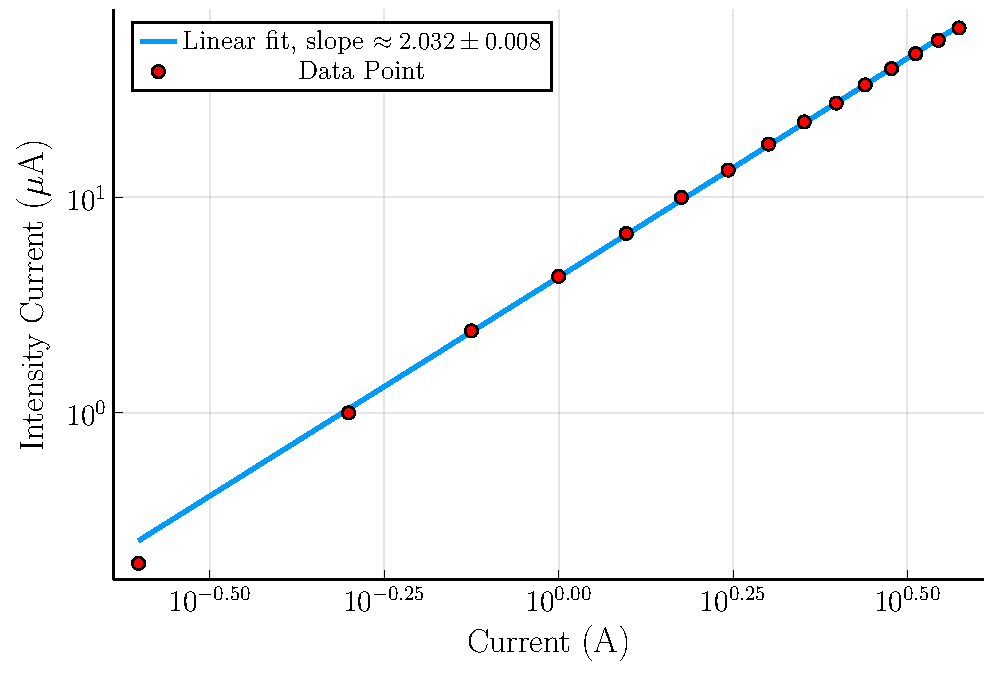
\includegraphics[width=0.7\textwidth]{malus.pdf}
    \caption{Intensity vs. Current in log-log scale with the linear fit shown with solid line.}
\end{figure}